\documentclass{article}
\usepackage[utf8]{inputenc}
\usepackage{tikz}
\usepackage[short,nodayofweek,level,12hr]{datetime} 

\title{Programmering for Matematikere 
\\ ---\\
Miniprojekt: Et lufthavnskø problem \\
\large Guide til statistik modellering}


\date{Aalborg Universitet, \today}
\author{T. Kallehauge, J. J. Nielsen}


\usepackage{color}
\usepackage{amsmath}
\usepackage{amssymb}
\usepackage{amsthm}
\usepackage[
%  disable, %turn off todonotes
 colorinlistoftodos, %enable a coloured square in the list of todos
 textwidth=\marginparwidth, %set the width of the todonotes
 textsize=scriptsize, %size of the text in the todonotes
 ]{todonotes}

\usepackage[a4paper, total={6in, 10in}]{geometry}
\setlength\parindent{0in}

\usepackage[english]{babel}
\usepackage{datetime}
\usepackage{graphicx}
\definecolor{suchblue}{RGB}{150, 255, 150}
\usepackage{float}
\usepackage{caption}
\usepackage{mathtools}
\newtheorem{theorem}{Theorem}
\newtheorem{corollary}{Corollary}[section]
\newtheorem{lemma}[section]{Lemma}
\newtheorem*{remark}{Remark}
\newtheorem{definition}{Definition}[section]
\newtheorem{proposition}{Proposition}[section]


\usepackage{algorithm}% http://ctan.org/pkg/algorithms
\usepackage{algorithmic}% http://ctan.org/pkg/algorithms
\newcommand{\pluseq}{\mathrel{+}=}
\DeclareMathOperator{\Var}{Var}
\usepackage{color}
\usepackage{hyperref}
\usepackage{tipa}
\usepackage{pgfplots}
\pgfplotsset{compat = 1.16}
\usepackage{footmisc}
\usepackage{listings}
\usepackage{tcolorbox}
\usepackage{enumitem}

\usepackage{array}
\usepackage{lmodern,babel,adjustbox,booktabs,multirow}
\usepackage[normalem]{ulem}


\renewcommand{\thefootnote}{[\arabic{footnote}]}
\newcommand{\mbf}[1]{\mathbf{#1}}
\newcommand{\mbs}[1]{\boldsymbol{#1}}
\newcommand{\mR}{\mathbb{R}}
\newcommand{\mE}{\mathbb{E}}
\newcommand{\mC}{\mathbb{C}}
\newcommand{\mZ}{\mathbb{Z}}
\newcommand{\mN}{\mathbb{N}}
\newcommand{\Tr}[1]{\Text{Tr}{\left(#1}\right)}
\newcommand{\norm}[1]{\left\lVert#1\right\rVert}
\newcommand*{\cond}{\hspace*{1pt} |\hspace*{1pt}}

\newcommand{\tobi}[1]{\todo[color=suchblue!40,author=Tobias]{#1}}

\DeclareMathOperator*{\argmax}{arg\,max}
\DeclareMathOperator*{\argmin}{arg\,min}
\DeclareMathOperator*{\Cov}{Cov}
\DeclareMathOperator*{\logit}{logit}

\lstdefinestyle{mystyle}{
    backgroundcolor=\color{lightgray},   
    basicstyle={\ttfamily\footnotesize}
}
\lstset{style=mystyle,breaklines=true}

\newcommand\NoIndent[1]{%
  \par\vbox{\parbox[t]{\linewidth}{#1}}%
}



\usepackage[backend=bibtex,
  bibencoding=utf8,
  sorting = nty, 
  ]{biblatex}



\addbibresource{mybib.bib}
\DeclareNameAlias{sortname}{last-first}
\DeclareNameAlias{default}{last-first}
\DefineBibliographyStrings{english}{%
   bibliography = {Bibliografi},
}	
\renewcommand*{\bibfont}{\small}

\begin{document}
\maketitle
\newpage
Dette dokument er supplement til det primære dokument omhandlende miniprojektet. I dette dokument bliver der givet en guide til hvordan man kan simulere ankomsttidspunkter og landingsvarighed set fra et \textit{statistiks} synspunkt. Da I på nuværende tidspunkt ikke har haft statistik, vil de nødvendige begreber gennemgås, men kun på overfladisk niveau. Guiden er primært matematisk. Der vil blive givet hints til hvordan tallene kan simuleres i Python, men det er i udgangspunktet op til jer at finde ud af. 
\section{Introduktion til sandsynlighed og fordelinger}
Kort sagt er et sandsynlighedsmål $P$ en funktion, der bestemmer sandsynligheden for hændelser $A$ som $P(A)$. $P$ er begrænset mellem $0$ og $1$. Eksempelvis er sandsynligheden for hændelsen \textit{slå en 6'er} med en 6-sidet terning $P(\text{slå en 6'er}) = 1/6 \approx 0.17\%$. \\
For at formalisere notationen i tilfældige forsøg,  eksempelvis at slå med en terning, indfører vi begrebet \textit{tilfældige variable}. En tilfældig variabel er en funktion $X: S \to\mR$, der får sine værdier fra et tilfældigt forsøg hvor $S$ er mængden af mulige udfald. I forsøget med terningen vil $X(\text{slå en 6'er}) = 6$, $X(\text{slå en 1'er}) = 1$, osv. Vi kan så skrive $P(X = 6) = 1/6$. Et andet eksempel er møntkast hvor den tilfældige variabel $X$ kan repræsentere antallet af kroner i løbet af 3 møntkast. Hver vil $X(PPK) = 1$, $X(KKP) = 2$, $X(KKK) = 3$ osv.
\\ \\
Med begrebet tilfældige variable kan vi indføre \textit{sandsynlighedsmassefunktionen}, på engelsk \textit{probability mass funktion} (pmf), som egentlig blot er en nemmere notations metode. En pmf $p_X$ er defineret som $p_X(x) = P(X = x)$ for en tilfældig variable $X$. Bemærk her at $X$ er den tilfældige variabel mens $x$ er et reelt tal, eksempelvis er $P(\text{slå en 6'er}) = P(X = 6) = p_X(6)$. 
\\ \\ 
Det viser sig at mange forsøg kan kategoriseres med parametriske \textit{fordelinger} med tilhørende pmf'er. Fra kursusgangen om tilfældige tal kender vi allerede et par fordelinger nemlig den \textit{uniforme fordeling}  og \textit{normalfordelingen}. Forsøget med terningslag er et eksempel på en uniform fordeling hvor $p_X(x) = 1/6$ for $x = 1,\dots, 6$, altså lige stor sandsynlighed for alle udfald. I terningslag forsøget følger $X$ altså en uniform fordeling med udfald mellem $1$ og $6$ og vi skriver $X \sim \text{unif}(1,6)$. Forsøget med terning og møntkast er eksempler på \textit{diskrete fordelinger}, da der er et tælleligt antal udfald i forsøget. Vi kan også have \textit{kontinuerte} fordelinger hvor man ikke kan tælle antal udfald, eksempelvis normalfordelingen hvor udfaldet kan være alle reelle tal. Ved kontinuerte fordelinger snakker man istedet for pdf'er om \textit{sandsynlighedstæthedsfunktioner}, på engelsk \textit{probability density function} (pdf). En uniform fordeling kan også være kontinuert hvis vi tillader alle reelle tal i et interval $[a,b]$ og vi har pdf funktionen $p_X(x) = 1/(b-a)$\footnote{I kontinuerte fordelinger skal man integrere for at udregne sandsynligheder. Vi har specielt at \\
 $P(a \leq X \leq b) = \int_a^b p_X(x)\ dx$. Eksempelvis har vi for en kontinuert uniform fordelingen mellem $0$ og $1$ at\\ $X \sim \text{unif}(0,1)$, $p_X(x) = 1$ og $P(0 \leq X \leq 0.5) = \int_0^{0.5} 1 \ dx = 0.5$.}.
% 
\section{Simulering af ankomsttidspunkter - Poisson proces}
De relevante oplysninger vi har fået at vide om lufthavnens trafik er:
\begin{itemize}
\item Der ankommer i gennemsnit $200$ fly om dagen, men på en given dag kan der både ankomme færre eller flere.
\item Trafikken ankommer indenfor en periode på $13$ timer. 
\item Ankomsttidspunkterne er tilfældige inden for perioden og ikke koordineret flyene imellem. 
\item Trafikken forventes at stige med $5\%$ om året fremover. 
\end{itemize}
Et sådant setup er klassisk indenfor modellering af systemer hvor begivenheder sker tilfældigt i tid. Lignende eksempler kunne være ankomst af opgaver til en computerserver, kø på apoteket, tidspunkter for jordskælv, ulykker på motervej og henfald af radioaktive partikler. Alle disse eksempler kalder man for \textit{punktprocesser} hvor tidsperioden mellem to hændelser er tilfældige variable $T_1, T_2,\dots$ som illustreret i figur \ref{fig:process1}. 
\begin{figure}
\centering
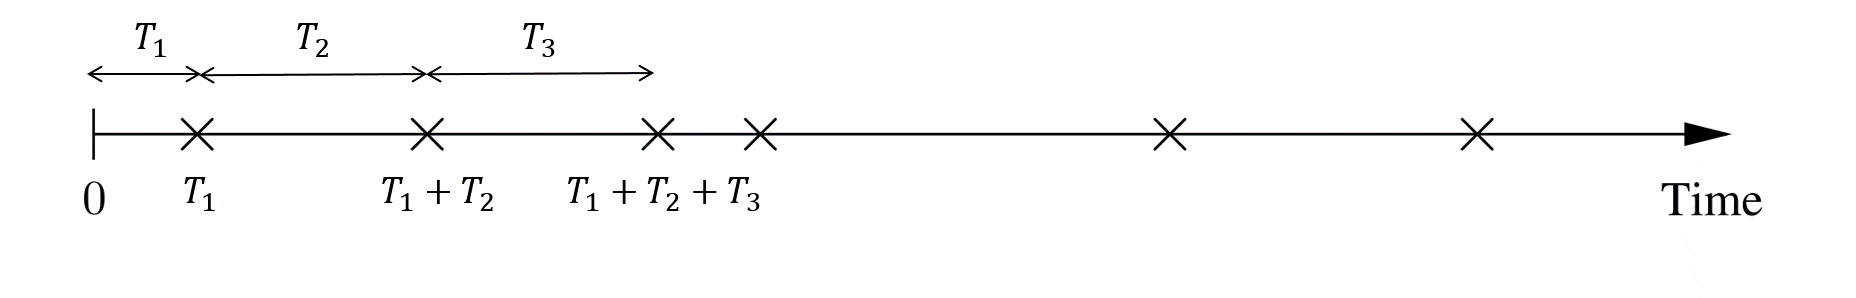
\includegraphics[width = \textwidth]{process1.png}
\caption{Punktprocess hvor $\times$ markerer hændelser i tid - eksempelvis ankomsttidspunkter af fly.} \label{fig:process1}
\end{figure}
Det viser sig, at når man antager uafhængighed mellem tidspunkter\footnote{Se \cite[123-127]{olofsson2012} for de præcise detaljer.}, da vil $T_1, T_2,\dots$ nødvendigvis følge en såkaldt \textit{eksponentielfordeling} med rate $\lambda$ og vi kalder punktprocessen for en \textit{Poisson process}. \\
En exponentielfordeling er en kontinuert fordeling og hvis $X$ følger en eksponentielfordeling med rate $\lambda$ da er pdf funktionen\footnote{Man kan simulere tal fra eksponentielfordelingen med \texttt{numpy.random.exponential} hvor man skal angive parametret \texttt{scale}. \texttt{scale} svarer til $\lambda^{-1}$}:
\begin{align*}
p_X(x) = \lambda e^{-\lambda x}, \quad x \geq 0,
\end{align*}
og vi skriver $X \sim \exp(\lambda)$ (se figur \ref{fig:distributions}). Raten $\lambda$ i eksponentielfordelingen har indflydelse på hvor hurtigt vi ser et udfald og en eksponentialtfordelt $X$ vil i gennemsnit have udfaldet $1/\lambda$. I en Poisson fordeling har vi altså at $T_i \sim \exp(\lambda)$ for $i = 1,2\dots,$ hvor hver $T_i$ har gennemsnit $1/\lambda$.
\\ \\
Følgende resultat om Possion processer er nyttigt. Lad $X(t)$ være en tilfældig variabel der tæller antallet af punkter fra $0$ til $t$ i en Poisson process med rate $\lambda$. Det viser sig da at $X(t)$ følger den såkaldte \textit{Possion fordeling} med parameteren $k = \lambda t$. En Poisson fordeling er en diskret fordeling og hvis $X$ følger en Poisson fordeling med parameter $k$ da er pmf funktionen\footnote{Man kan simulere tal fra Poissonfordelingen med \texttt{np.random.poisson} hvor man skal angive parameteret \texttt{lamb}. \texttt{lamb} svarer til $k$.}
\begin{align*}
p_X(x) = e^{-k}\frac{k^x}{x!}, \quad x = 0,1,\dots
\end{align*}

\begin{figure}
\centering
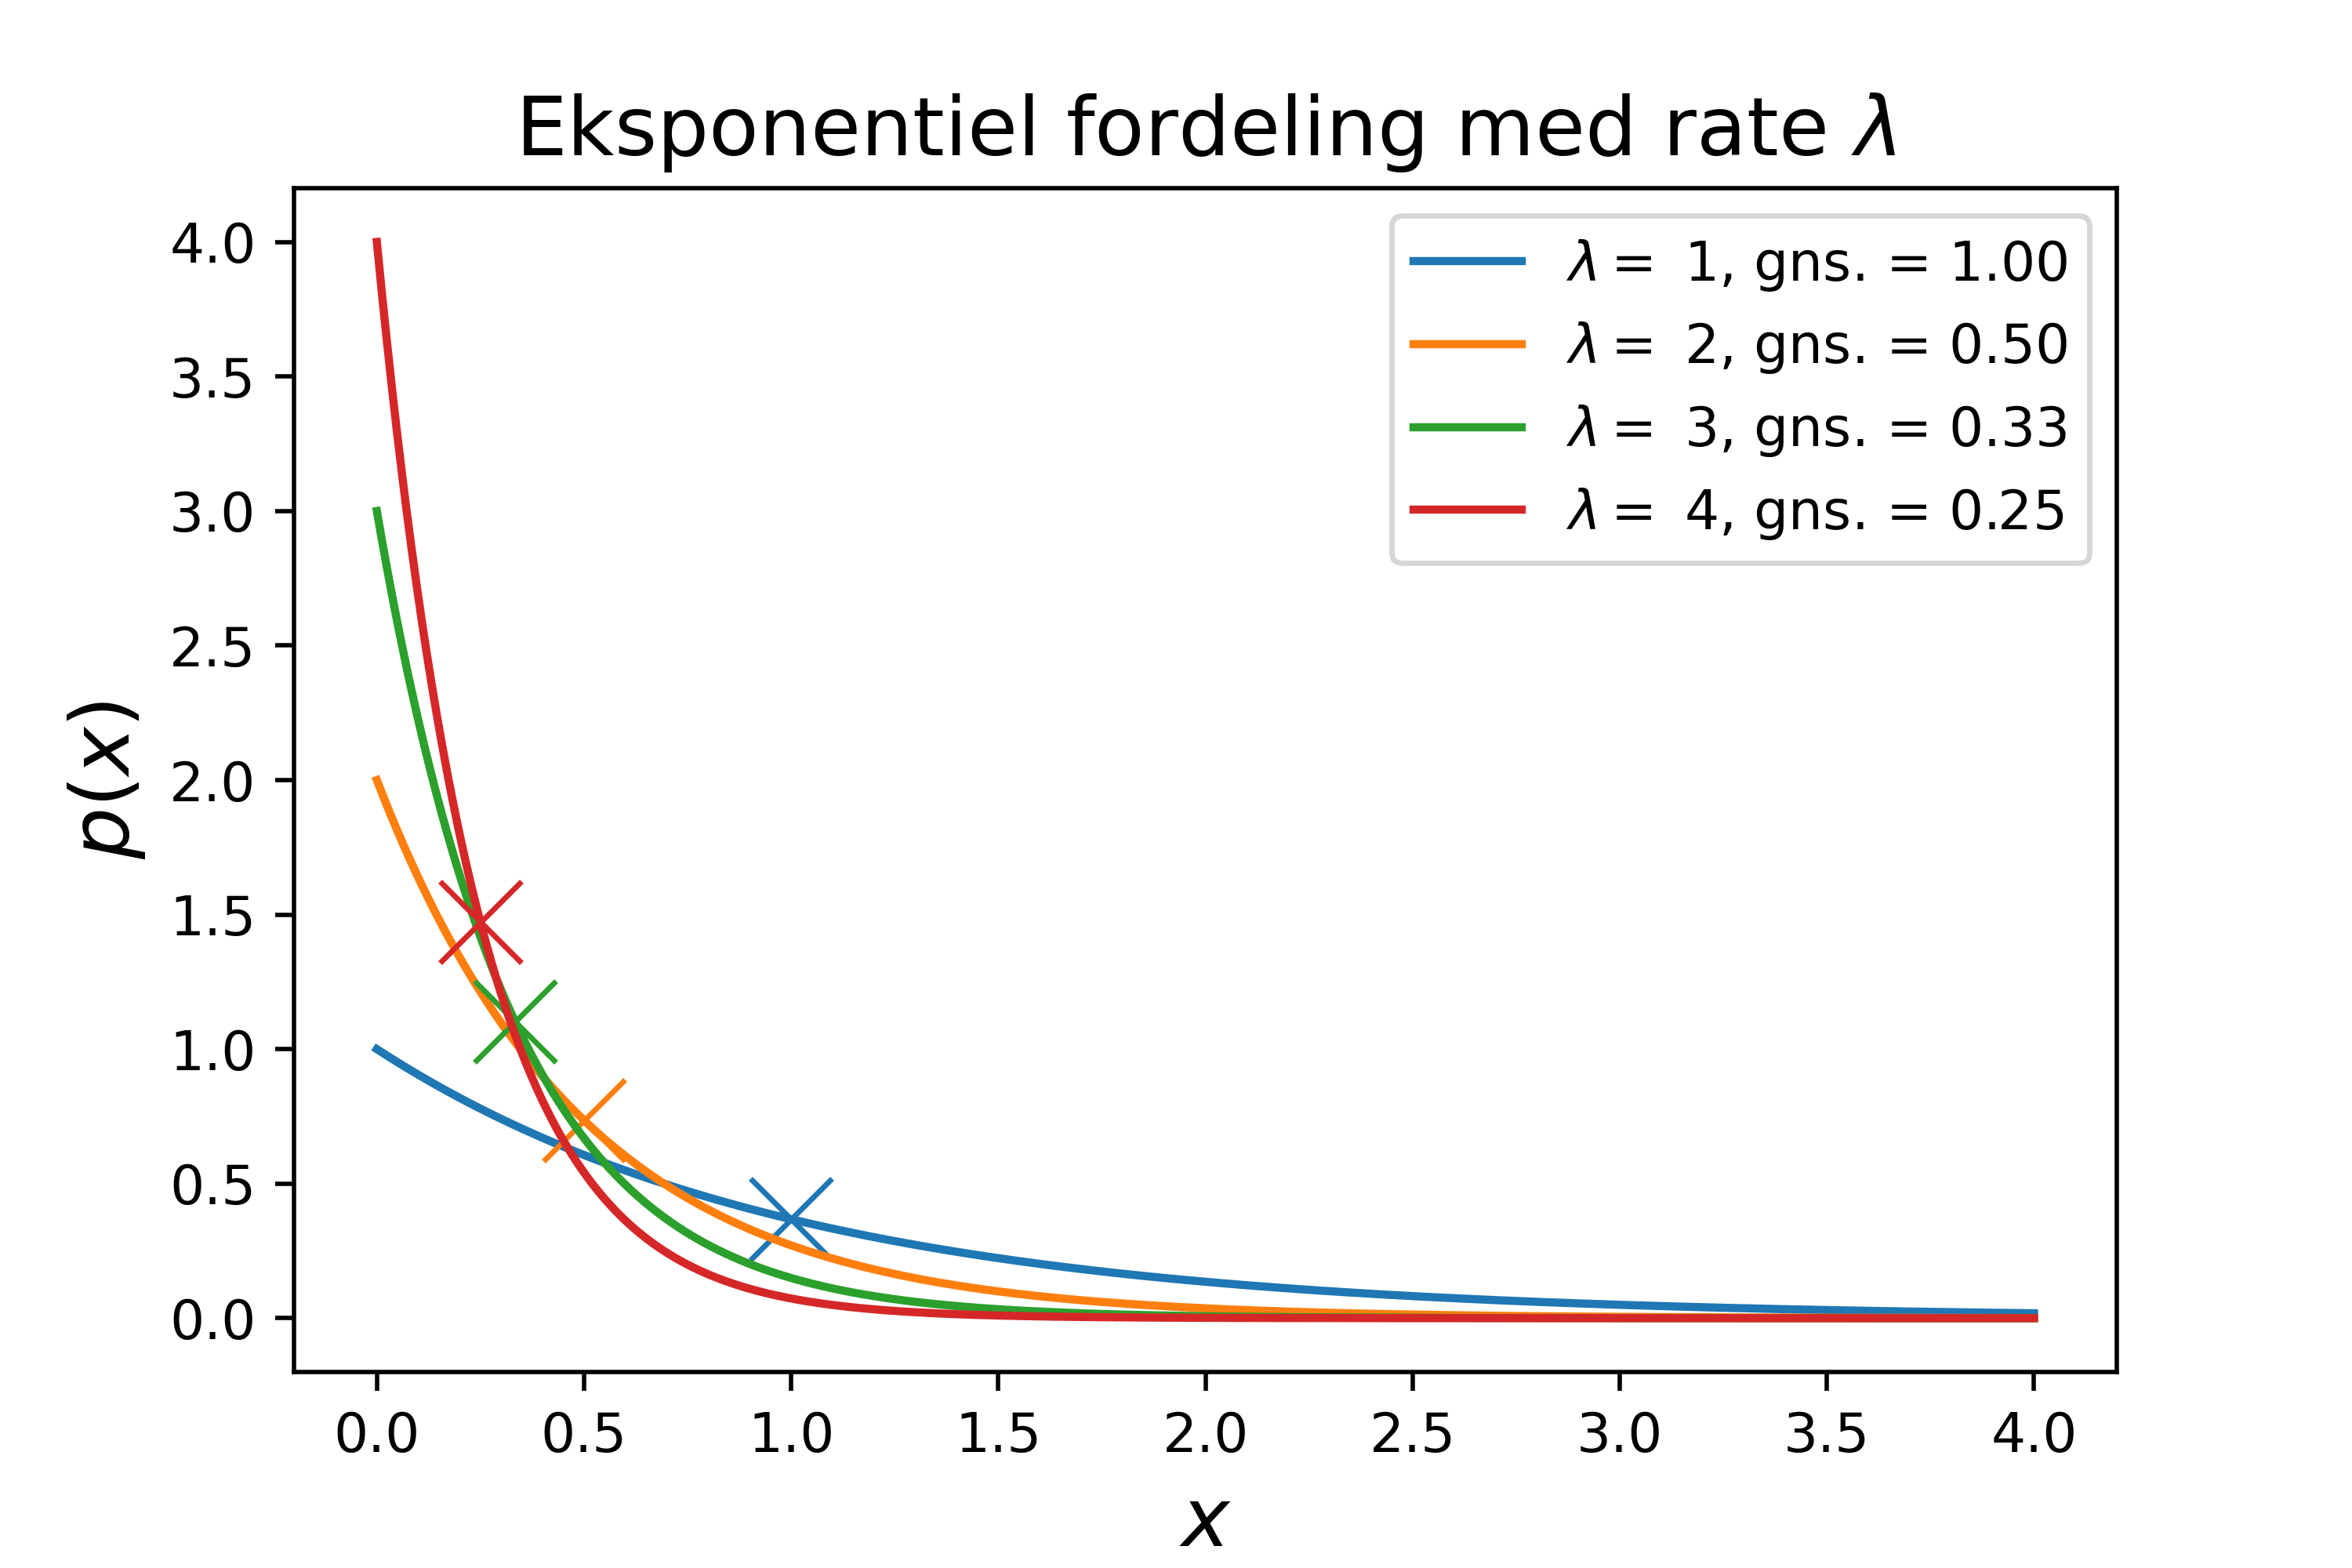
\includegraphics[width = 0.45\textwidth]{exp_dist.png}
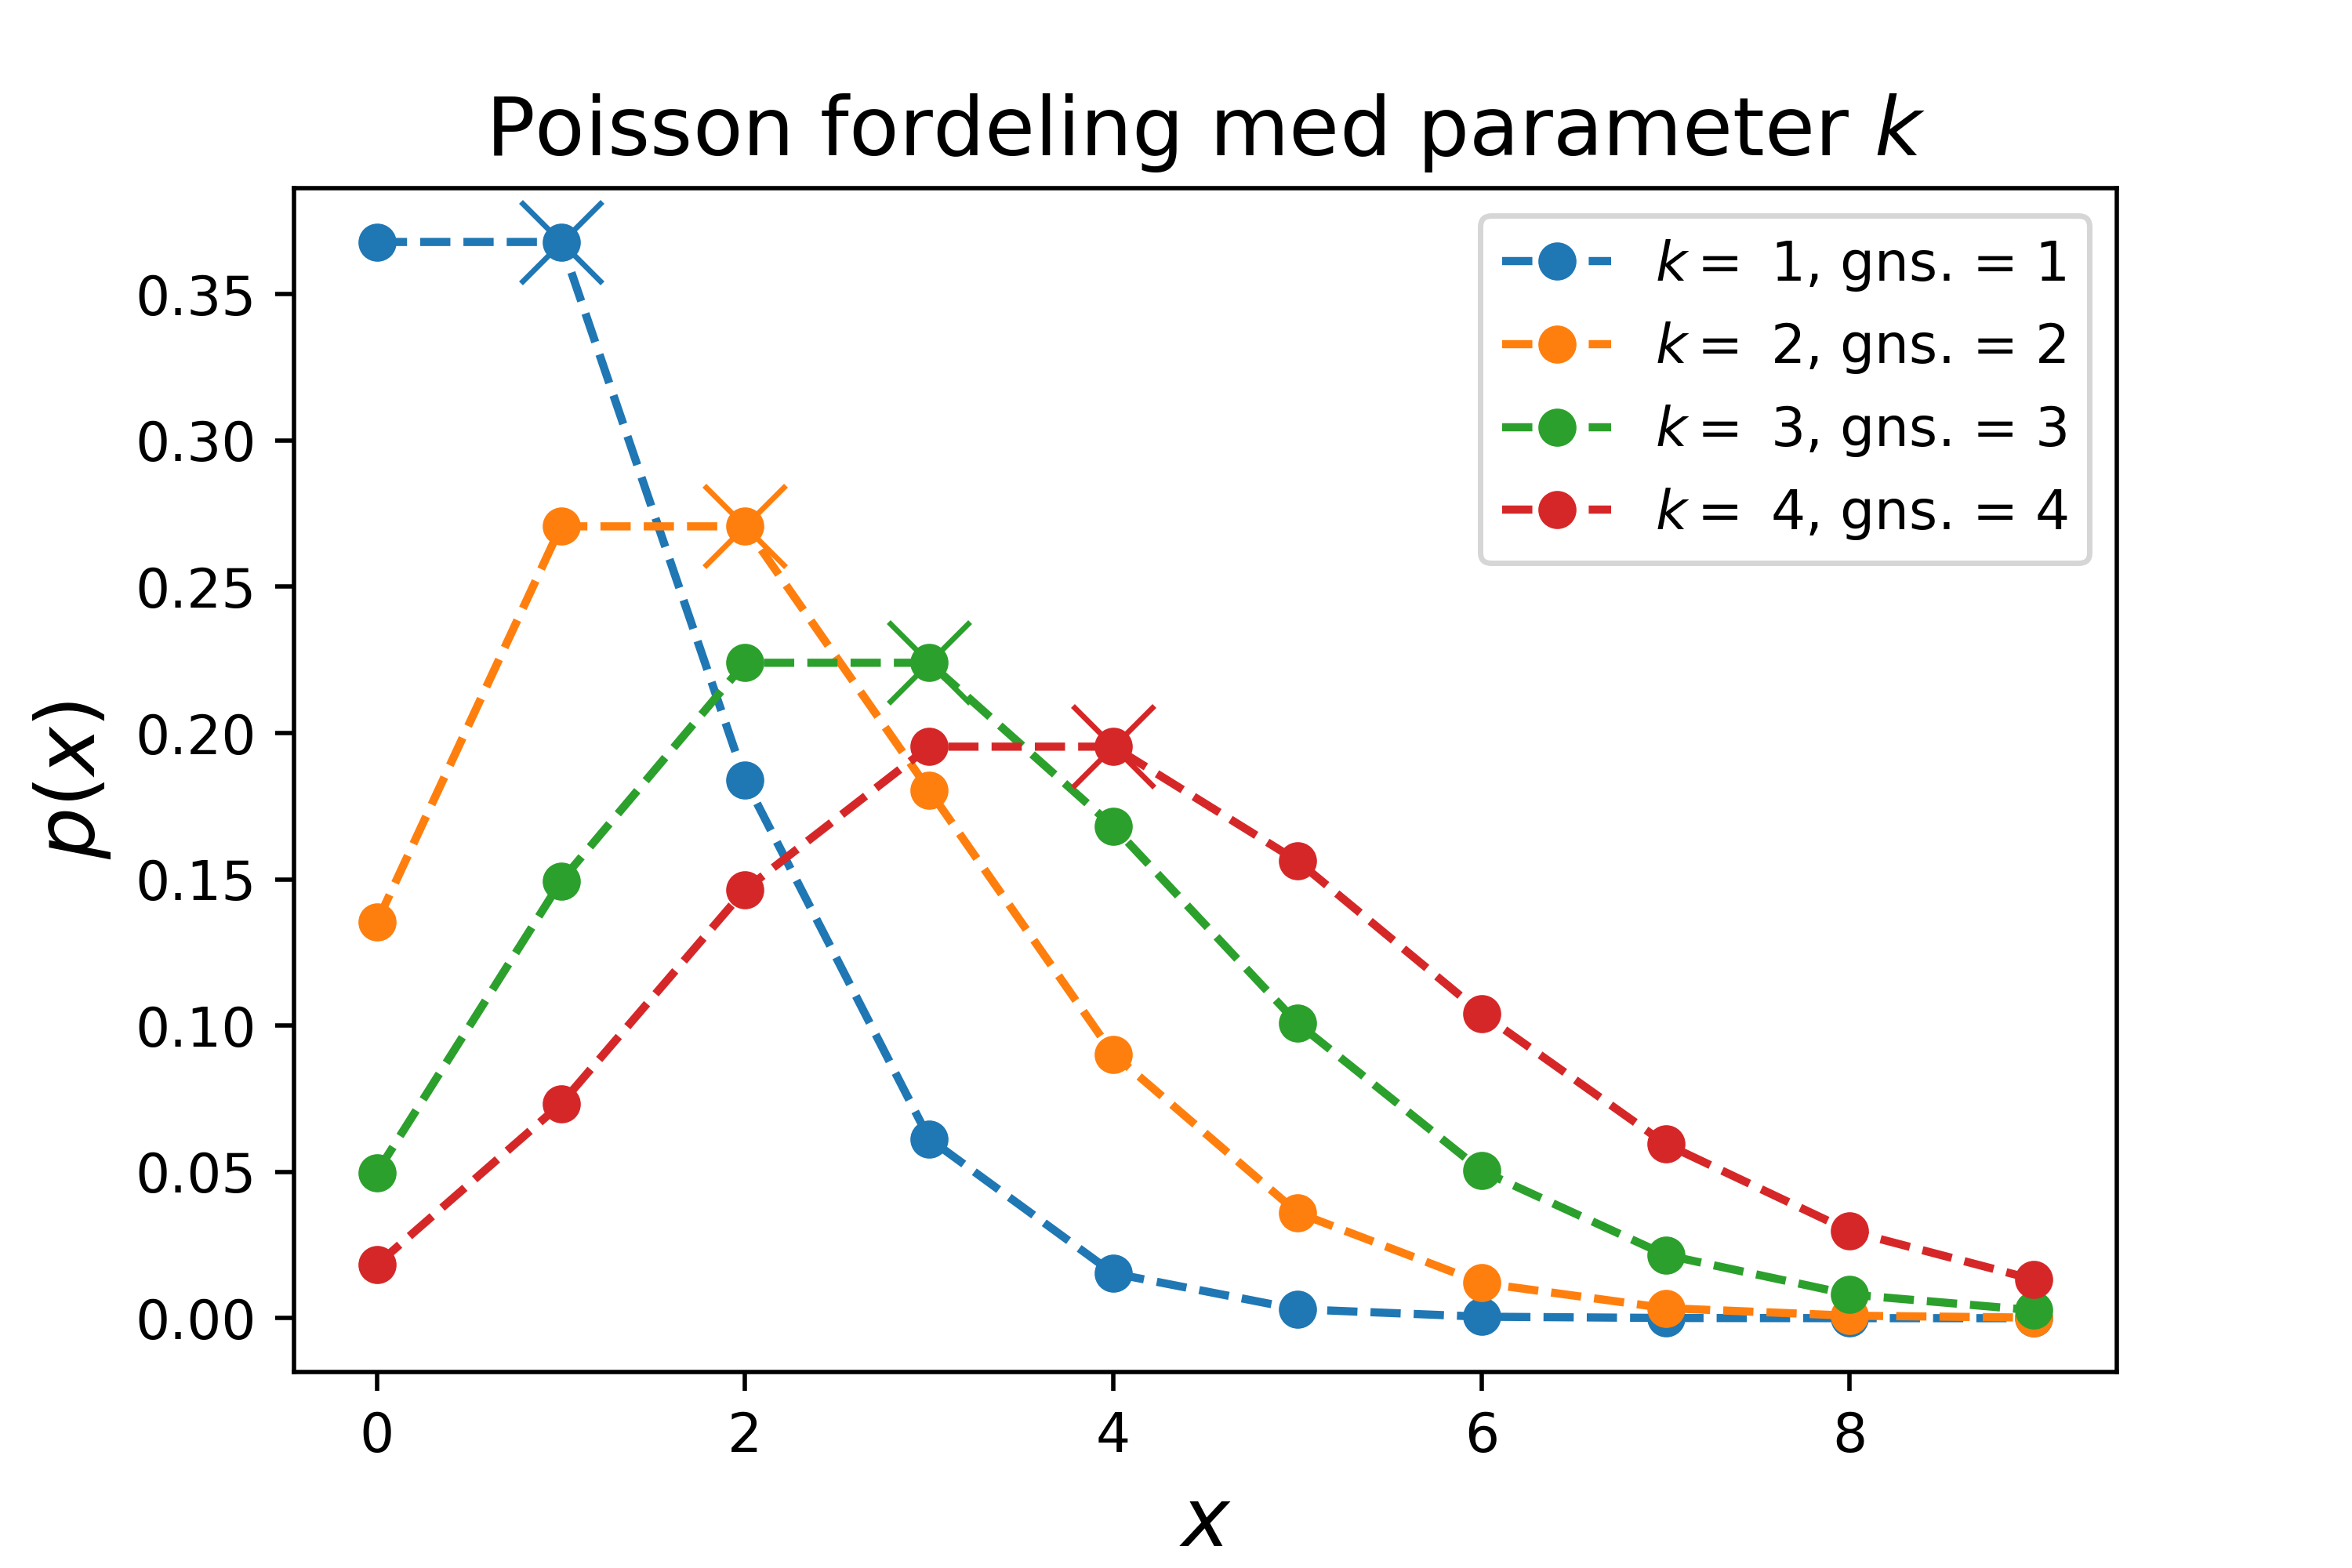
\includegraphics[width = 0.45\textwidth]{poiss_dist.png}
\caption{pdf og pmf for eksponentiel og Poisson fordeling. $\times$ markerer gennemsnit ved de forskellige parametre.} \label{fig:distributions}
\end{figure}
Den gennemsnitlige værdi af en Poisson fordeling med parameter $k$ er blot $k$ (se figur \ref{fig:distributions}). Lad os se på følgende eksempel: En Possson process har rate $\lambda = 2$. Ud fra resultatet vil antal punkter ved $t = 10$ sekunder være Poisson fordelt med parameter $k = 20$ og vi forventer gennemsnitligt $20$ punkter ved $t = 10$. 
\\ \\
Et sidste nyttigt resultat kan bruges til nemt at simulere en Poisson process. Vi har givet en Poisson process med rate $\lambda$. Givet at der er $N$ antal punkter i tidsperioden $[0,t]$ vil fordelingen for tidspunkterne være uafhængigt uniformt fordelte tilfældige variable i intervallet $[0,t]$. Kender vi $N$ kan man altså blot simulere $N$ punkter uniformt fordelt i intervallet $[0,t]$ for at simulere en Poisson process.
\\ \\
I kan læse mere om eksponentielfordelinger, Poissonfordelinger og Poisson processer i \cite{olofsson2012} (online version er gratis tilgængelig på AUB). Heri finder i også beviser for resultaterne om Poisson processen. Ovenstående er dog til tilstrækkeligt til at generere de tal vi skal bruge i miniprojektet. Overvej følgende spørgsmål for at simulere ankomsttidspunkter af fly: 
\begin{itemize}
\item Hvordan kan man bestemme rate parametren $\lambda$ ud fra de givne oplysninger? 
\item Hvordan kan man simulere antal fly på en dag?
\item Hvordan kan man simulere ankomsttidspunkter givet antal fly på en dag?  
\item Hvordan kan effekten af stigende trafik på $5\%$ om året simuleres? Hint: Brug $\lambda$. 
\end{itemize}

\section{Ikke-parametriske fordelinger og simulering af landings\-varig\-hed}
Til landingstiderne har vi fået oplyst en række tidsintervaller og hvor mange flys landingsvarigheder, der typisk falder inden for hvert interval. I dette afsnit lærer vi teorien til hvordan disse oplysninger kan bruges til at generere tilfældige landingsvarigheder i overensstemmelse med de givne oplysninger.  
\\ \\
Eksponentielfordelingen var et eksempel på en parametrisk fordeling hvor blot ét enkelt tal, $\lambda$, karakteriserer hele fordelingen. Fordelingen for landingsvarighed er dog en smule mere kompliceret da mange parametre såsom flytype og vejrforhold har indflydelse. Så i stedet for at prøve at finde en tilpas kompliceret fordeling, der passer på data, kan vi tilpasse en \textit{ikke parametrisk} fordeling direkte ud fra data. Den nemmeste metode til dette er følgende. Lad intervallet $[a,b]$ være udfaldsrummet for en tilfældig variabel $X$ og lad $I_1 = [a,x_1), I_2 = [x_1,x_2)\dots, I_N = [x_{N-1},b]$ være $N$ delmængder, der dækker intervallet. Lad os nu antage at vi har en række observationer af $X$, og definer da størrelsen:
\begin{align*}
p_i = \frac{n_i}{\Delta_iM},
\end{align*}
hvor $n_i$ er antallet af observerede punkter inden for det $i$'te interval, $\Delta_i$ er størrelsen på hvert interval og $M$ er det total antal observationer. Følgende funktion er da en ikke parametrisk pdf for det observerede data:
\begin{align*}
p_X(x) = \begin{cases}
p_1 & x \in I_1 \\
p_2 & x \in I_2 \\
\vdots \\
p_N & x \in I_N \\
0 & x \notin [a,b]
\end{cases}
\end{align*}
Eksempel: Vi har observeret følgende dataset med $20$ observationer:
$$\vec{x} = \left(2.4,\hspace{1pt} 3.8,\hspace{1pt} 2.8,\hspace{1pt} 2.4,\hspace{1pt} 1.7,\hspace{1pt} 3.1,\hspace{1pt} 1.7,\hspace{1pt} 6.7,\hspace{1pt} 9.9,\hspace{1pt} 1.5,\hspace{1pt} 4.7,\hspace{1pt} 2.3,\hspace{1pt} 2.5,\hspace{1pt} 7.8,\hspace{1pt} 0.2,\hspace{1pt} 0.3,\hspace{1pt} 0.1,\hspace{1pt} 5.4,\hspace{1pt} 4.5,\hspace{1pt} 6.1 \right)$$
Inddeles intervallet $[0,10]$ i $[0,2), [2,4), \dots, [8,10]$ fås således:
\begin{align*}
\vec{nr} &= (6,\hspace{1pt} 7,\hspace{1pt} 3,\hspace{1pt} 3,\hspace{1pt} 1), \quad \Delta = 2, \quad M = 20 \quad \text{og} \\
p_X(x) &= \begin{cases}
\frac{6}{2\cdot 20} & x \in [0,2) \\
\frac{7}{2\cdot 20} & x \in [2,4) \\
\frac{3}{2\cdot 20} & x \in [4,6) \\
\frac{3}{2\cdot 20} & x \in [6,8) \\
\frac{1}{2\cdot 20} & x \in [8,10] \\
0 & x \notin [0,10]
\end{cases},
\end{align*}
illustreret i figur \ref{fig:ikke_para_pdf}. 
\begin{figure}[H]
\centering
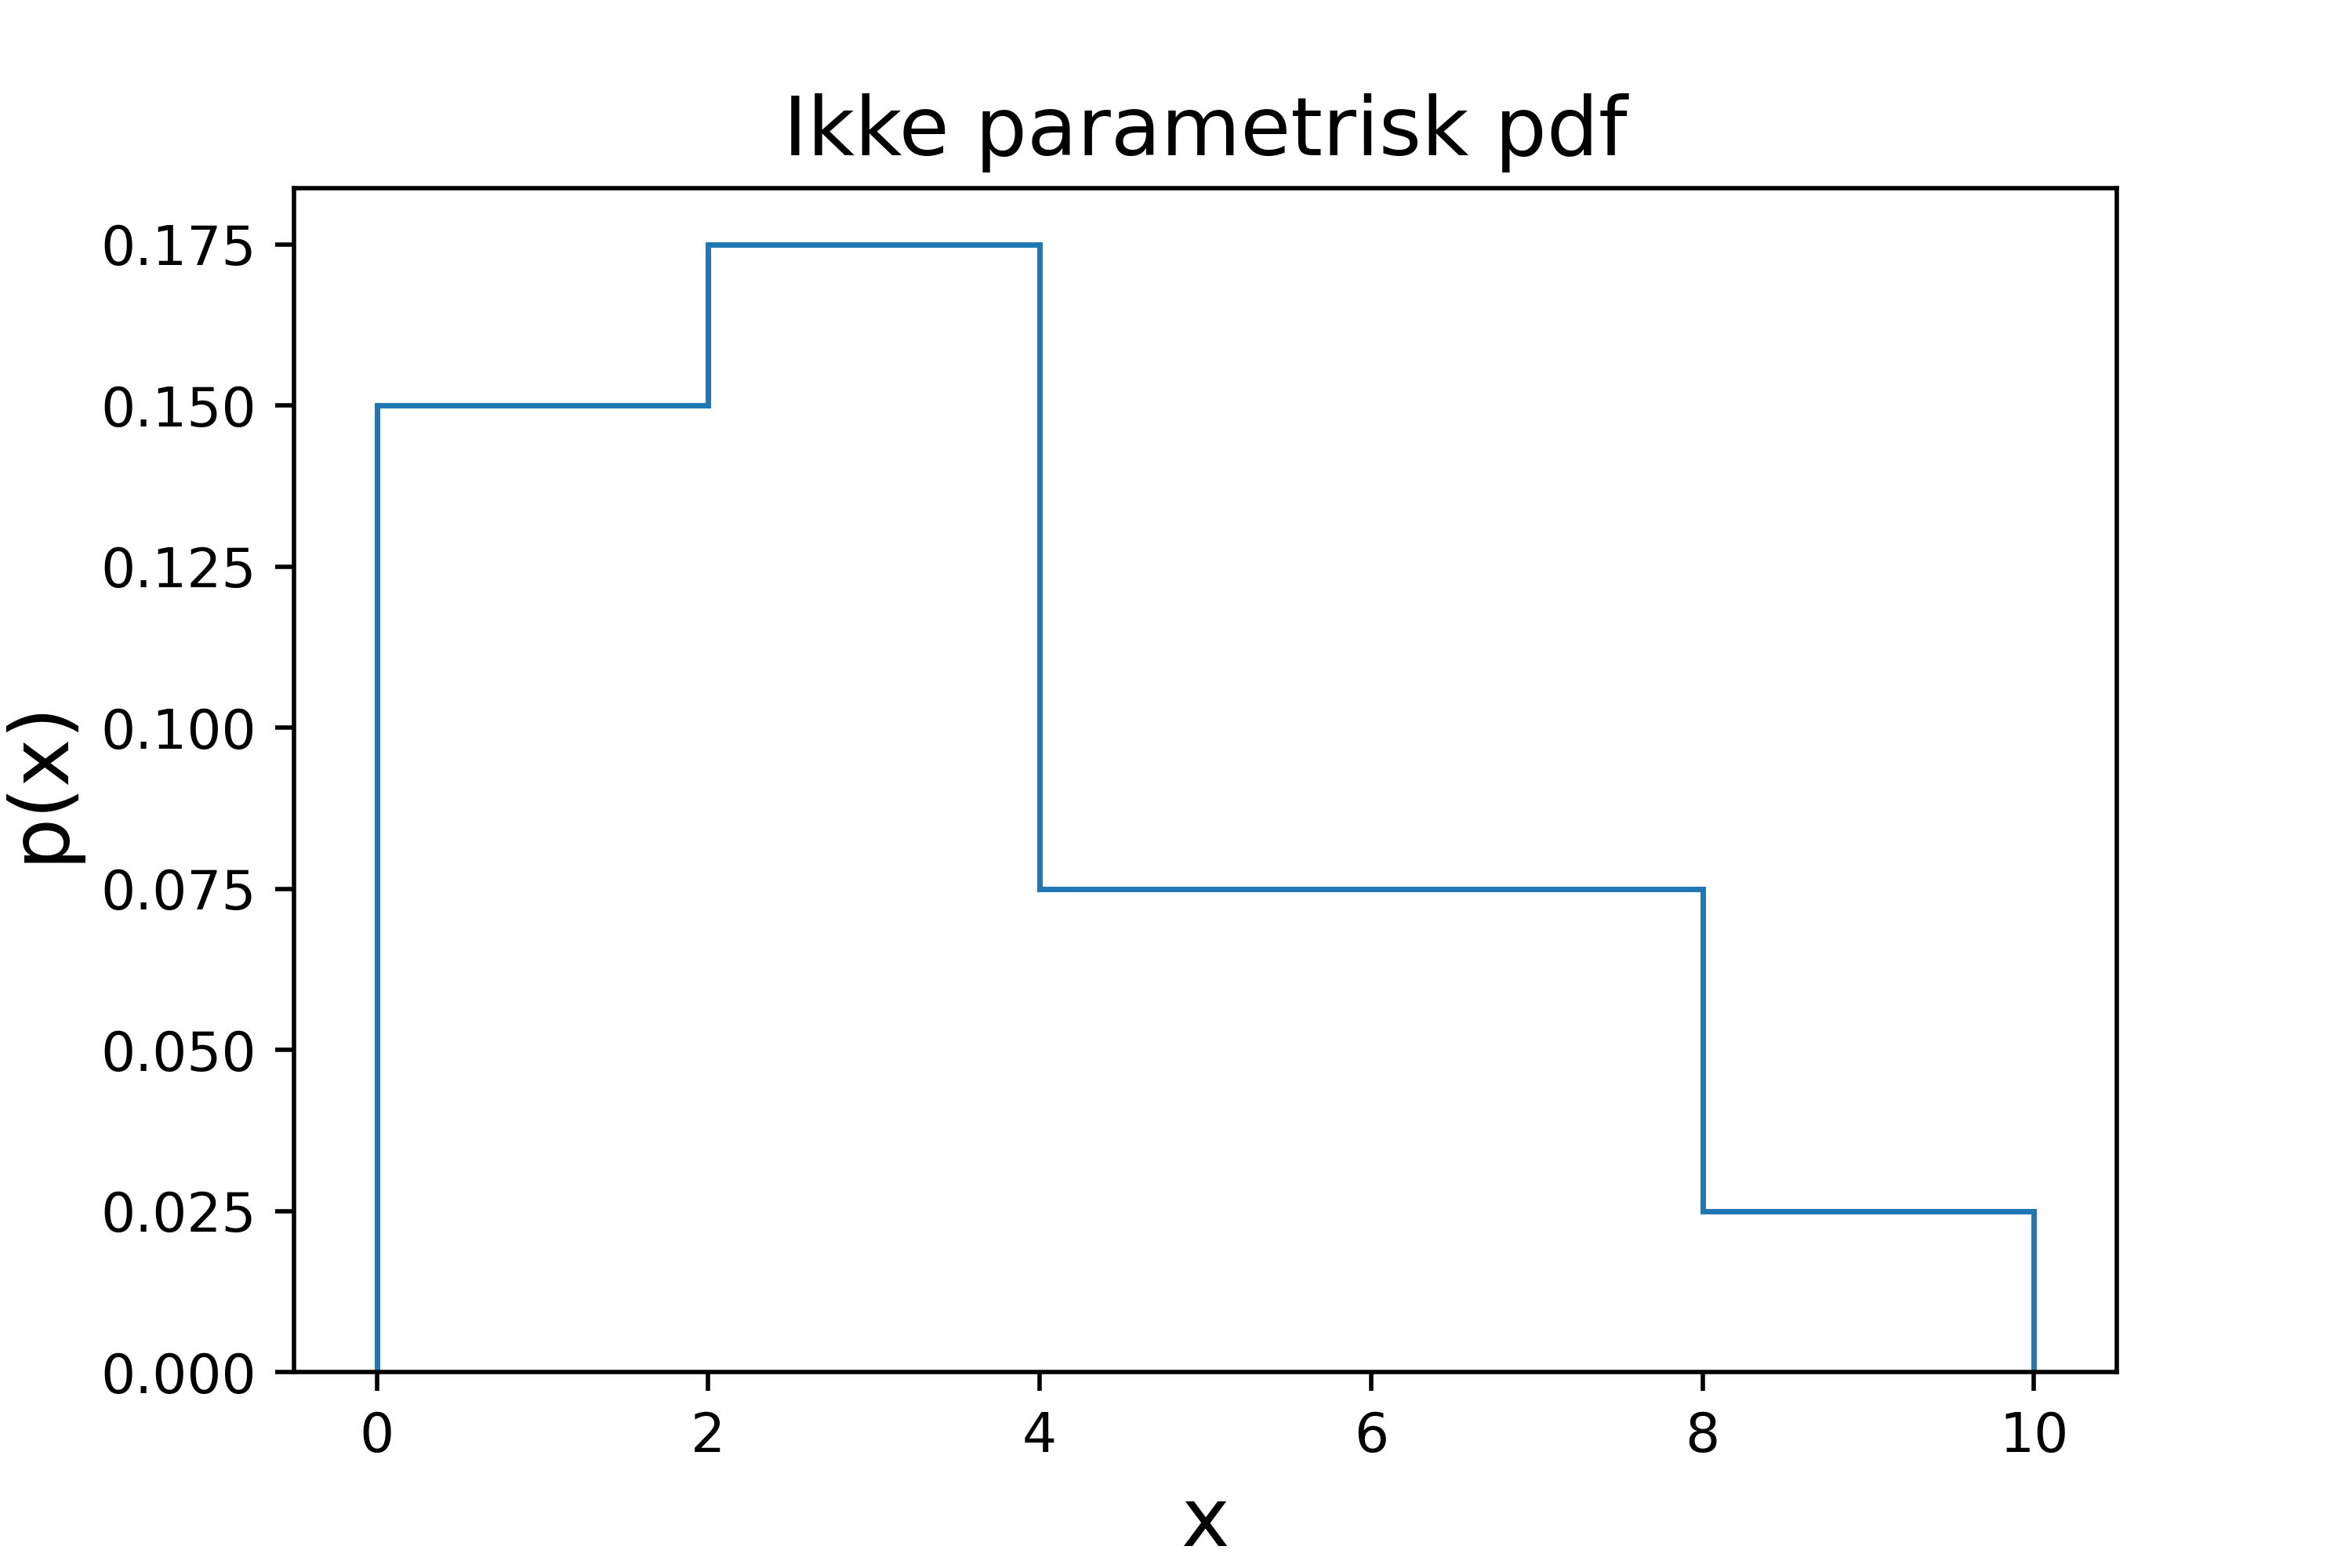
\includegraphics[width = 0.45\textwidth]{ikke_para_pdf.png}
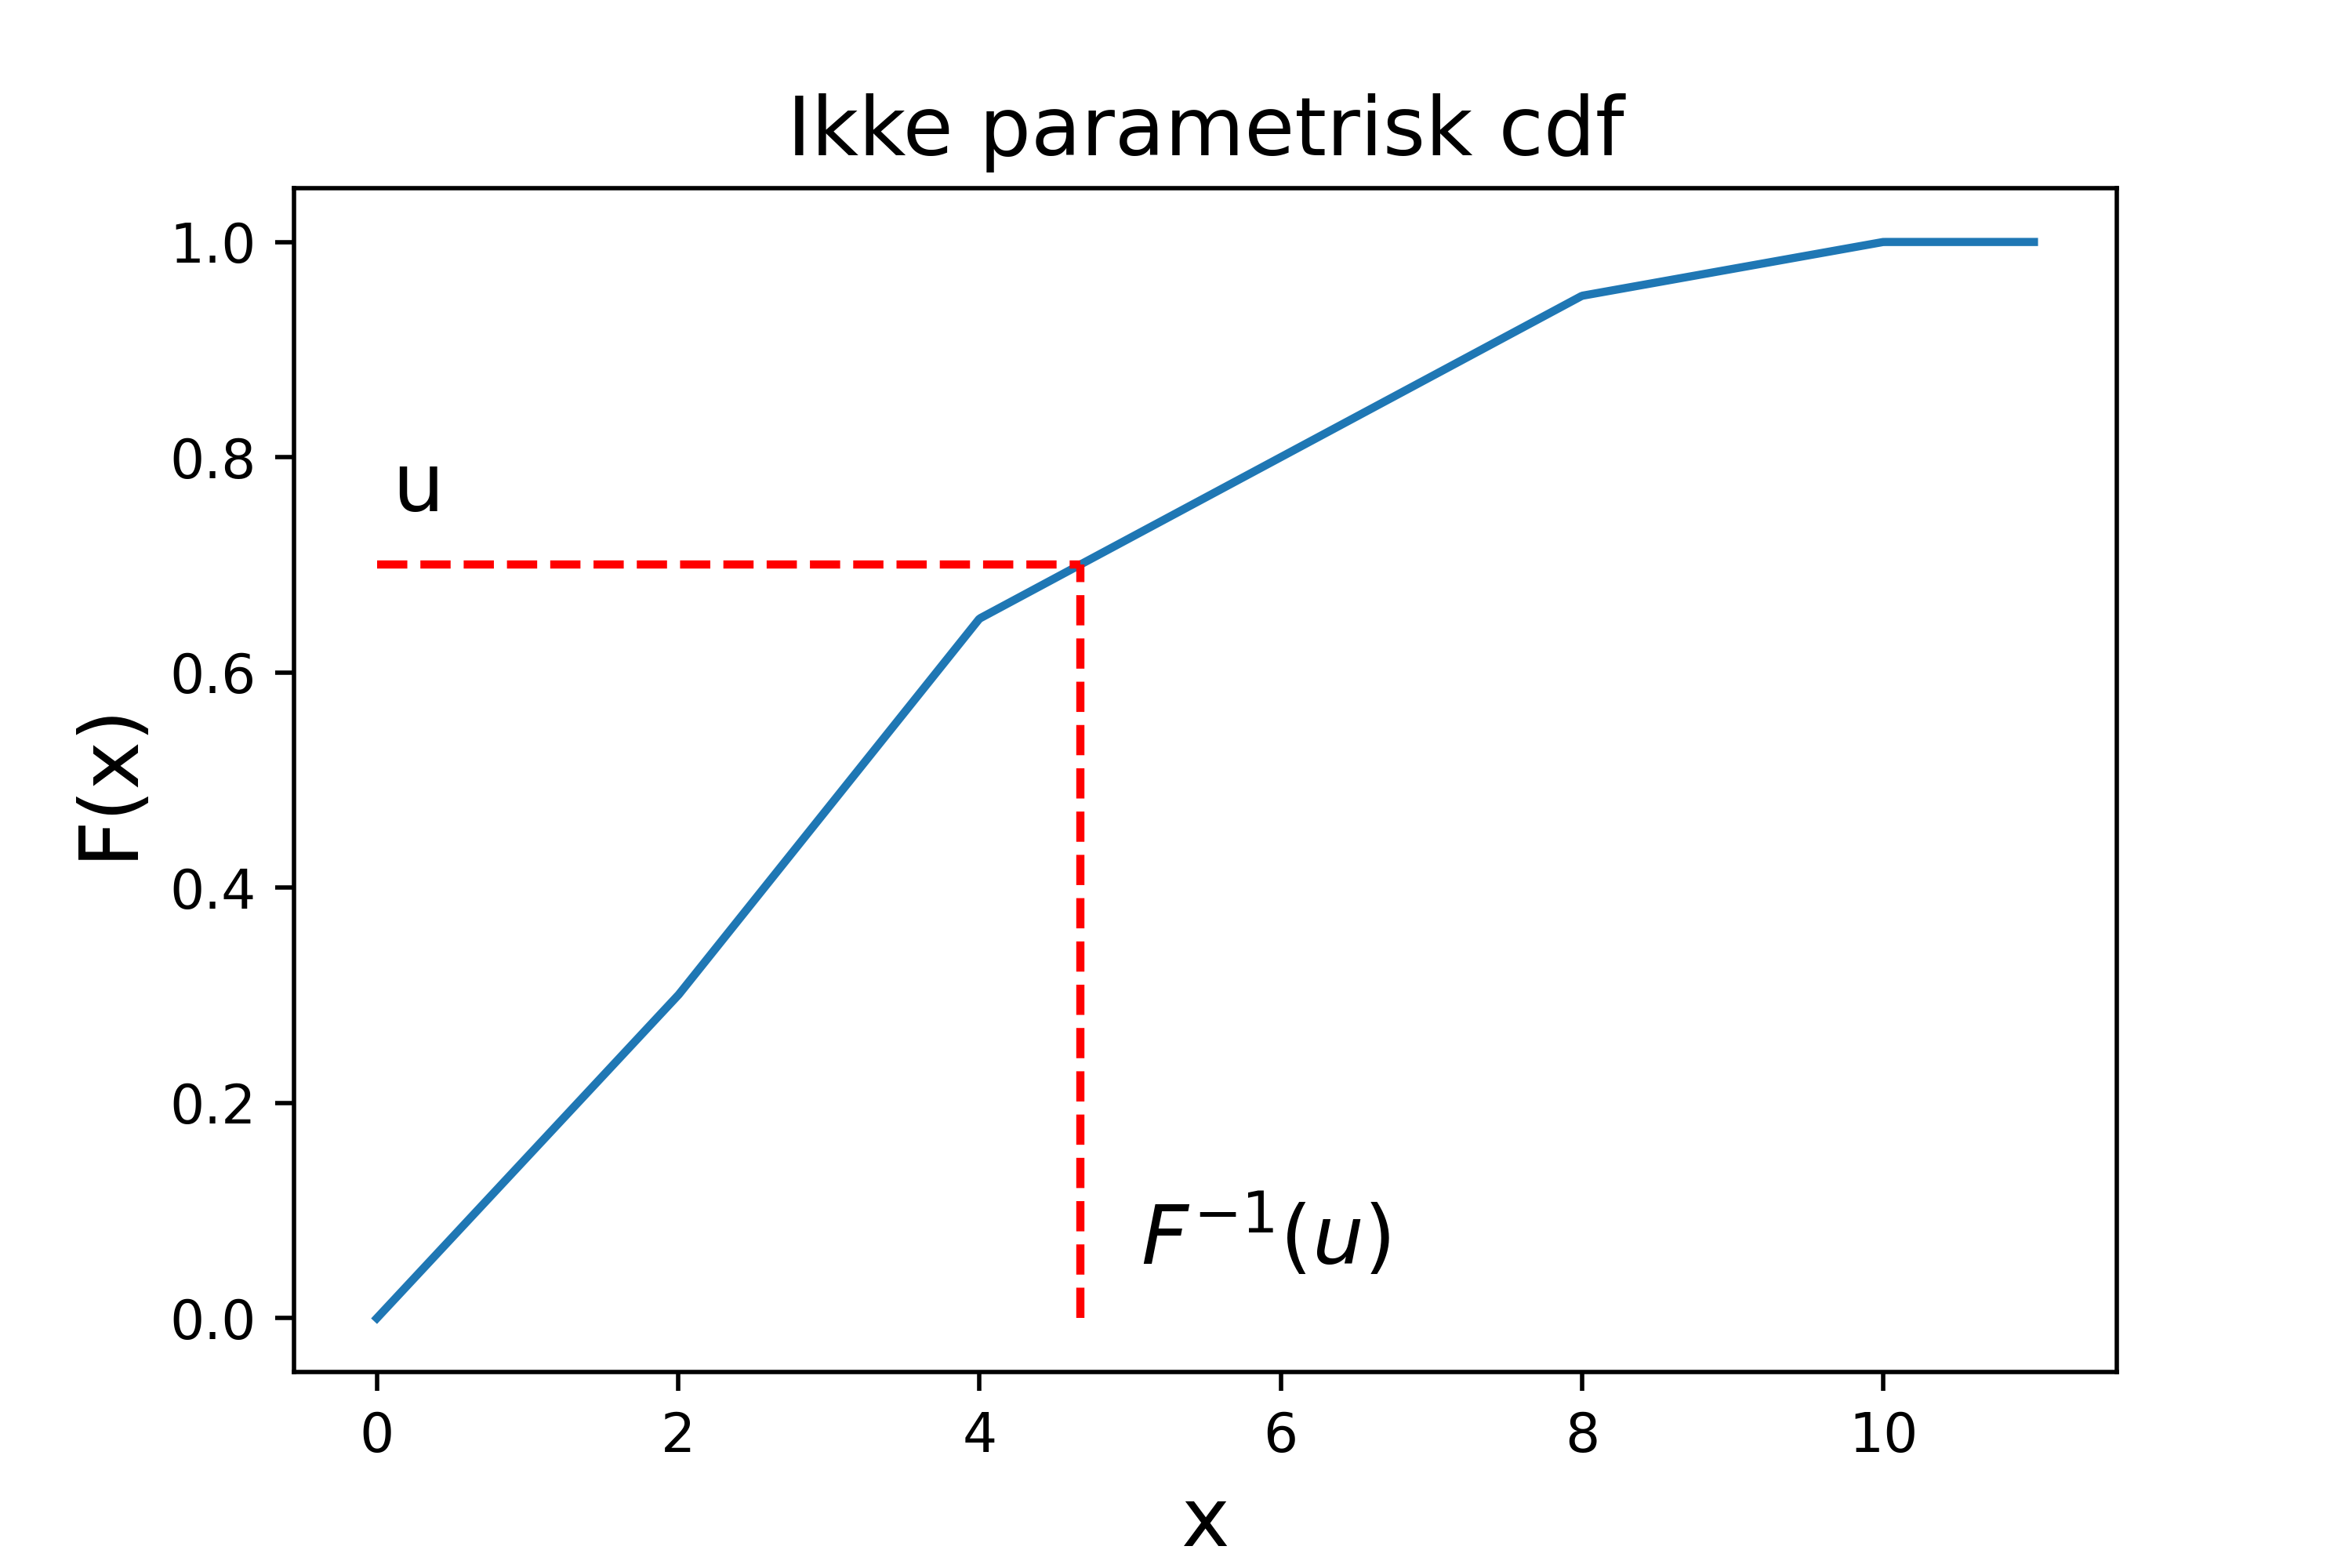
\includegraphics[width = 0.45\textwidth]{ikke_para_cdf.png}
\caption{Ikke parametrisk pdf og cdf for eksemplet med 20 observationer.} \label{fig:ikke_para_pdf}
\end{figure}
For at simulere tal givet en pdf kan man bruge den \textit{inverse cdf metode}. En cdf er den kumulative fordelings funktion eller på engelsk cumulative distribution function, og denne beskriver sandsynligheden for at en tilfældig variabel er mindre end eller lig en bestemt værdi. For en tilfældig variabel $X$ noteres cdf'en typisk $F_X$, og der gælder at $F_X(x) = P(X \leq x)$. For kontinuerte fordelinger kan man udregne CDF'en ved at integrere pdf'en via:
\begin{align*}
F_X(x) = \int_{-\infty}^{x} p_X(x) \ dx
\end{align*}
Givet en cdf kan man udtrække tal fra den fordeling den stammer fra ved følgende to skridt:
\begin{itemize}
\item Udtræk et tilfældigt tal $u$ fra en uniform fordeling mellem $0$ og $1$. 
\item Sæt $x = F_X^{-1}(u)$ hvor $F_X^{-1}$ er den inverse cdf for $X$ (givet at den eksisterer). $x$ vil da følge fordelingen for $X$.
\end{itemize}
Dette koncept er illustreret i figur \ref{fig:ikke_para_pdf}. 
\\ \\
Ovenstående kan bruges til at simulere mange fordelinger, men i vores tilfælde kan det være en smule besværligt at integrere sig frem til $F_X$ og derefter at finde den inverse funktion $F_X^{-1}$. I det specifikke tilfælde hvor vi har en ikke parametrisk pdf, der er uniformt fordelt i nogle bestemte intervaller, kan vi simulere tal fra fordelingen på følgende vis:
\begin{itemize}
\item Vi har igen delt udfaldsrummet $[a,b]$ op i $N$ intervaller$$I_1 = [a,x_1),\ I_2 = [x_1,x_2),\ \dots,\ I_N = [x_{N-1},b]$$
\item Udregn blot cdf'en i højresiden af de valgte intervaller altså $F_X(x_1), F_X(x_2), \dots, F_X(x_N)$ hvor $x_N = b$. \\
Hint: $F_X(x_1), F_X(x_2), \dots, F_X(x_N)$ har en særlig simpel form når vi kender $p_1, \dots, p_N$. Lav udledningen på tavlen. 
\item Udtræk et tilfældigt tal $u$ uniformt fordelt mellem $0$ og $1$. 
\item Find det mindste interval $I_i$ således $u \geq F_X(x_i)$, altså $I_i$ hvor $i = \min\left\{i \cond u \geq F_X(x_i) \right\}$. 
\item Simuler $x$ fra en uniform fordeling i intervallet $I_i$. 
\end{itemize}
Med en velvalgt illustration kan man overbevise sig selv om at ovenstående metode er ækvivalent med invers cdf metoden når vi har en pdf, der består af en række flade intervaller. Der er selvfølgelig mange andre metoder man kan bruge, som i meget gerne må undersøge, men ovenstående er tilstrækkeligt for miniprojektet til simulering af  landingstider. Overvej følgende hjælpespørgsmål:
\begin{itemize}
\item Hvordan kan vi bruge oplysningerne i miniprojektet til at udregne $p_i$ værdierne? 
\item Hvordan kan vi udregne $F_X(x_i)$ værdierne ud fra $p_i$ værdierne? 
\item Hvordan kan vi simulere tilfældige landingsvarigheder givet ovenstående? 
\end{itemize} 

\printbibliography[heading=bibintoc]
\label{bib:mybiblio}
\end{document}